\label{sec:evolutionarystaghunt}
Evolutionary games consist of a population of agents that are randomly matched 
over time to play a stage game. In an evolutionary interpretation of the
stag hunt game, it is repeatedly played as the stage game.
Usually, the number of agents is assumed to be (infinitely) large, 
such that on one hand, the effect of a single individual 
on the population is small, and on 
other hand, the interaction happens anonymously.
Furthermore, agents are described as myopically, so that they do not 
discount later payoffs.
Populations can either be \textit{monomorphic} or \textit{polymorphic}.
Monomorphic populations consist of agents that are only able to play pure
strategies, whereas in polymorphic populations mixed strategies are allowed.
In the following, the focus will be on monomorphic populations as they have
a straightforward interpretation and the main implications do not differ. 
Formally, let $p_j(t) \geq 0$ denote the number of individuals in 
the population playing strategy $j \in \{1,2\}$ at time $t \in \realnumb$ and 
let $P = p(t) = p_1(t) + p_2(t)$ describe the total number of all individuals 
in the population. Note, $P =p(t)\ \forall t$ meaning that the population 
is not growing. The vector $\vec{x}(t) = \left(x_1(t),x_2(t)\right)^T
=\left(\frac{p_1(t)}{p(t)},\frac{p_2(t)}{p(t)}\right)^T$ is called the state 
vector of the population at time $t \in \realnumb$. 
Each component of the population state vector represents the share of agents 
choosing a specific strategy. As the individuals can only choose between 
strategy 1 and 2 in the SH game, it holds that  $x_2(t) = 1-x_1(t)$. 
Mentioned earlier, a stage game played by a population enables a 
new interpretation of mixed strategies, because $\vec{x}(t)$ is an 
element of the mixed strategy space $\Delta$ for all $t$.
Hence, mixed strategies in monomorphic games are simply the state
of the population, which is the division of players on the two
pure strategies in the SH game. 
This has, however, little relevance for the interpretation
in the traditional game \parencite[914-915]{rubinstein_comments_1991}.

Out of convenience, let the expected payoff 
to a strategy $j \in \{1,2\}$ of an individual randomly matched
against another individual in the current population state $\vec{x}(t)$ 
at time $t$ be denoted by $F^j(\vec{x}) = \hat{F}(e_j,\vec{x}(t))$. 

\subsection{Revision Protocols}
\label{sec:revisionprotocols}
This section motivates the use of revision protocols to
model the behavior of agents.
In contrast to the traditional approach, agents in evolutionary game theory 
are usually neither able to calculate best-replies, 
nor are they observing the information relevant
to perform the necessary calculations.
Revision protocols formalize the idea that agents are following a certain
rule by which they change their strategy. 
The following derivation is by \textcite{sandholm_population_2010}. 
Typically it is assumed that agents have an inner alarm clock 
which rings at a rate R following an exponential distribution. 
Of course, this does not translate 
in economic applications to individuals having literal clocks around their
wrist, but illustrates the idea of a randomly occuring chance to reconsider
their strategy choice.
The agents' clocks are assumed to be independent of each other, such that
the individuals chance to revise does not dependent on others.
Whenever the clock of an agent rings, he
receives a revision opportunity which means that he changes his strategy
with the probability $\frac{\rho_{ij}}{R}$, where
$\rho_{ij}(\hat{F},\vec{x}(t))$ is called the conditional switch rate,
representing the rule by which agents change from strategy 
$i$ to strategy $j$. The conditional switch rate usually depends
on the current state of the population $\vec{x}(t)$ at time $t$ and the
mixed strategy payoff function of the underlying game $\hat{F}$.
In a two-strategy game there are two conditional switch rates, $\rho_{12}$ 
describing the rate of switching from strategy 1 to 2 and $\rho_{21}$, 
the rate for switching from strategy 2 to 1. For $\rho_{ii}$ no actual switch 
happens.
Switch rates result in different individual behavior rules, and furthermore 
in different dynamics for the whole population. An evolutionary
dynamic describes the change of the population vector $\vec{x}(t)$ in time. 
The derivation of the dynamic can be done for a general conditional switch 
rate. 
Every agent receives $R dt$ revision opportunities, i.e.\ the clock rings, 
in a time interval $[0,dt]$ as it follows a Poisson distribution with
mean $Rdt$ \parencite[123]{sandholm_population_2010}. 
If the population in the stag hunt game is at state $\vec{x}(t)$, the number 
of agents currently playing strategy $i$ receiving a revision opportunity 
during the time interval of length $dt$ is $Px_i R dt$. As 
\textcite{sandholm_population_2010} argues, this is an approximation because
the state of the population $\vec{x}(t)$ may change during the time interval $dt$.
With the probability for an agent playing strategy $i$ switching to strategy
$j$, one gets $P x_i \rho_{ij} dt$ for the expected number of 
switches for strategy $i$ during $[0,dt]$ across the population.   
In a game with two strategies, the change in the number 
of agents in the population playing strategy 1 is determined 
by agents switching to strategy 2 and agents with strategy 2 
switching to 1. Hence, this leads to
\begin{align} 
        Pdx_1 =  \underbrace{-Px_1 \rho_{12}dt}_{\text{Switches from 1 to 2}} 
        + \underbrace{Px_2 \rho_{21}dt.}_{\text{Switches from 2 to 1}}
\end{align}
Dividing by $P$ and $dt$ yields the differential equation for
the change in the share of agents playing strategy 1, 
$\dot{x}_1 =\frac{dx_1}{dt}$. 
The sum of the time derivatives of population shares must equal zero and so
$\dot{x}_2(t) =- \dot{x}_1(t)$.
There are different plausible revision protocols studied in the literature. 
\textcite{sandholm_population_2010} discusses various forms of 
these revision protocols, such as logit choice, comparison to average payoff 
and best response protocol. 
They all contain different assumptions about the information 
an individual agent can obtain and about the abillity of the agents 
to process this information. Hence, the resulting evolutionary 
dynamics have different properties.

With respect to the implied dynamic, the 
\textit{pairwise proportional imitation} protocol will be outlined 
hereafter.  
It assumes that whenever an
agent receives a revision opportunity, he randomly gets to know 
another agent's strategy and its payoff received in the current 
state of the population. 
The switching probability of an agent choosing strategy $i$  
is proportional to the difference between the observed payoff $F^j(\vec{x})$ 
of the other agent with strategy $j$ and his payoff $F^i(\vec{x}})$.
This can formally be expressed as
\begin{align}
        \label{eq:pairwiseproportionalimitation}
        p_{ij} =
                \begin{cases}
                        x_j\left[F^j(\vec{x}) -F^i(\vec{x})\right] &\ ,
                        \text{for } F^j(\vec{x}) - F^i(\vec{x}) > 0 \\
                        0 &\ , \text{else}.
                \end{cases}
\end{align}
A story of traders on a marketplace can be told to illustrate this revision
protocol.
Suppose the traders interact on a market selling some 
good. They implicitly play a game with each other as their choice influences
the earnings of the others. The strategies may be the
way they organize their market stall or what position on the market they 
choose. Usually each trader does not
observe the strategies other traders use to sell things, because the market
place is large and the bustle going on is complicated. 
Hence, a trader is usually committed to a strategy he got to know a while ago.
As he returns to his tavern, he occasionally 
gets to meet another trader.
Being proud of their earnings, they boast about their 
individual strategy. In this way, they get to know
other traders' strategies and as they all dream of a live in pageantry,
they might imitate the other traders. 
However, they are more likely to imitate traders with a higher payoff 
compared to theirs, because such traders feel superior and thus, are the 
loudest in the tavern. 

Plugging the conditional switch rate of the pairwise imitation protocol 
\eqref{eq:pairwiseproportionalimitation} into the equation for the change 
of the population share playing strategy 1, $\dot{x}_1(t)$, leads to the 
\textit{replicator dynamic}:
\begin{alignat*}{2}
        \dot{x}_1 &= 2 x_1 x_2 \left[F^1(\vec{x}) - F^2(\vec{x})\right] \\
                  &= 2 x_1 \left[(1-x_1) F^1(\vec{x}) - x_2 F^2(\vec{x})\right] \\
                  &= 2 x_1 \left[F^1(\vec{x}) - \bar{F}(\vec{x})\right], \numberthis \label{eq:replicatorrev} 
\end{alignat*}
with the average payoff across the population 
$\bar{F}(\vec{x}) = x_1 F^1(\vec{x}) + x_2 F^2(\vec{x})$.
This equation fully describes the evolution of the population in time.
Properties and the connection to the stage game are discussed in the next
section.

\subsection{Replicator Dynamic}
\label{sec:replicatordynamic}
The replicator dynamic, one of the most popular dynamics in 
evolutionary game theory, has a wide range of applications and 
attractive properties, such as population genetics, ecology, abiogenesis, and
of course game theory \parencite[203]{hofbauer_evolutionary_1998}. 
It was mathematically formulated by \textcite{taylor_evolutionary_1978} and 
termed after the biological concept of a replicator, which was 
introduced in 1982 by Dawkins as the ``fundamental unit[s] of natural selection,
the basic thing[s] that survive or fail to survive''
\parencite[254]{dawkins_selfish_2016}. In a purely game theoretical fashion,
strategies are the replicators as they are propagated through the population
based on the revision protocol. Using the matrix notation, 
the replicator dynamic  
for the strategies $j \in \{1,2\}$ can be formulated as 
\begin{alignat}{2}
        \dot{x}_j &= x_j\left[\left(A\vec{x}\right)_j -
        \left(\vec{x}^T A \vec{x}\right)\right]. 
        \label{eq:replicator}
\end{alignat}
The first term in the bracket $(A\vec{x})_j$ is the expected payoff to 
strategy $j$ against the current population state at time $t$. The second
term is the average payoff of the whole population 
$(\vec{x}^T A \vec{x}) =\bar{F}(\vec{x})$.
The growth of the share $\dot{x}_j(t)$ at time $t$ depends 
on the share of the population currently using strategy $j$ and the 
excess payoff of that strategy, the difference between the expected 
payoff to strategy $j$ against the current state of the population and the
average payoff for the whole population.
Intuitively, the share of a strategy in the population increases (decreases) 
if the strategy yields a higher (lower) than average payoff. 
An evolutionary dynamic that satisfies this property is called 
\textit{payoff monotone} \parencite[30]{szabo_evolutionary_2007}. 
Comparing equation \eqref{eq:replicator} with equation 
\eqref{eq:replicatorrev}, one notices the lack of the factor $2$. 
This is simple due to the derivation of equation \eqref{eq:replicatorrev}.
In fact, any positive transformation of the payoff matrix 
results only in a change in speed of the replicator dynamic
\parencite[73]{weibull_evolutionary_1997}.
Another property of the replicator dynamic is the low data requirement.
Seen in the previous section, it was not 
necessary to assume that agents have much knowledge about the game or
the population. It was sufficient to assume that an agent gets to know the 
payoff of one random player. This is interesting for applications where it
is reasonable to assume that players cannot obtain much information.

Contrary to the interpretation that agents following a revision protocol 
are "boundedly rational", \textcite{gintis_game_2000}  argues 
that ``this is very misleading, because the real issue is the 
distribution of the information'' \parencite[273]{gintis_game_2000}. 
He claims, that even if they were not ``bounded'' they 
could not calculate a best-reply since they do not have the information about
the state of the population. For clarification, consider a representative
agent in the population. At time $t$ he plays strategy 1 and hence he
has an expected payoff $F^1(\vec{x})=\alpha_1 x_1$. But he actually receives 
either the payoff $\alpha_1$ or $\alpha_2$ when matched against another agent
with strategy $1$ or $2$, respectively. Based on that information and the
knowledge of another agents payoff, the agent
cannot deduce the composition of the population which is needed to choose
a strategy that maximizes the expected payoff. However, one can qualify this 
argument by assuming that agents have the information but cannot process it.
In the trader analogy, traders might be able to see the difference of the
other traders' stalls, but cannot recognize the secret of their success 
without others telling them.

A further property of the replicator dynamic is the lack of mutation or 
an error. In other words, a strategy that has not existed or has 
vanished from the population will not be in a future state of the population. 
That means, if only a subset $S' \subset S$ of the 
set of pure strategies is used in a population state, 
any future population state can also only contain strategies 
from this subset $S'$. Hence, if a strategy in 
the stag hunt game vanishes, the population state is in one of the two pure 
Nash equilbria. For further use it is practical to express the replicator 
dynamics for the parametrized SH game using the matrix in equation 
\eqref{eq:matrix} and define $x_1(t) := x,\ x_2(t) = 1-x$:
\begin{alignat*}{2}
        \dot{x} := \varphi(x) &= x^2(a-c+2d-2b) - x^3(a-c+d-b) -x(d-b) \\
                              &= x^2(\alpha_1+2\alpha_2) 
        - x^3(\alpha_1+\alpha_2) - x(\alpha_2) \numberthis
        \label{eq:replicatorpara}
\end{alignat*}
The last step follows by using local shifts on the matrix $A$. 
This does not change the dynamic at all because it preserves the relative
difference of payoffs \parencite[73]{weibull_evolutionary_1997}. 
The polynominal $\varphi(x)$ is
of degree $3$ and contains all information about the dynamic. Actually, 
as outlined below, it shows to which state the population converges.
In figure \ref{fig:polynominal} the graph of $\varphi(x)$ for the parameters
$a=5, b=0,c=4,d=3$ is shown. The ordinate represents the polynominal and
the abscissa represents the population share choosing strategy 1. Hence it is
between $0$ and $1$. Roots of the polynominal are the values of $x$ for 
which $\varphi(x)$ crosses the horizontal dashed gray line. The vertical
dashed gray line indicates the inner root, the root for an $x \in (0,1)$. 

\begin{figure}[h]
        \centering
        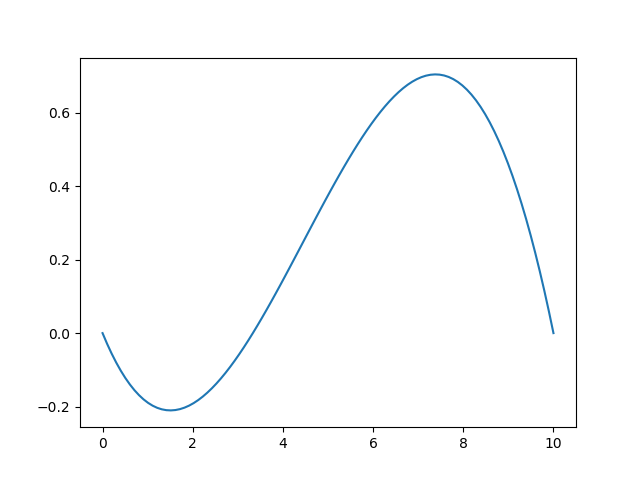
\includegraphics[scale=0.5]{polynominal.pdf}
        \caption[Polynominal of the Replicator Dynamic]{$\varphi(x)$ for the parameter setting $a=5, b=0, c=4, d=3$}
        \label{fig:polynominal}
\end{figure}
A solution through an initial state $x_0$ of the dynamical system is called a 
\textit{trajectory}, whereby it is distinguished between a forward trajectory 
for $t \rightarrow \infty$ and backward trajectory for $t \leftarrow \infty$.
Analytical solutions, i.e.\ solutions one can express with the use of
basic functions, can only be derived for simple cases. 
However, the existence and uniqueness of a solution through
any initial state for the replicator dynamic is guaranteed by the theorem 
of \textit{Picard-Lindel\"of}, theorem 6.1 in 
\textcite[74]{weibull_evolutionary_1997}. 

Once a solution is obtained, the question whether there 
is a connection between the evolutionary dynamic and the equilibria in the 
stage game arises. To see this, consider the concept of a fixed point.
A point $\vec{x}^*=(x^*_1,x^*_2)^T \in \realnumb^2$ of a dynamical system, such as the replicator 
dynamic in equation \eqref{eq:replicator}, is called a fixed point
if $\dot{\vec{x}} = 0$ at $\vec{x}^*$ , i.e.\ it stays in the 
current state for all $t \rightarrow + \infty $. 
Analyzing equation \eqref{eq:replicator}, 
this happens if either a strategy
is not present in the population or the excess payoff of a strategy is zero. 
Consequently, considering equation \eqref{eq:replicatorpara}, in the stag 
hunt game a fixed point can be characterized by an $x^*$ for which
$\varphi(x^*) = 0$.
The fixed points of the dynamic coincide 
with the Nash equilibria of the stage game as 
$\varphi(x^*) = 0$ for $x^* \in \{0,\frac{\alpha_2}{\alpha_1+\alpha_2},1\}$. 
It suffices to calculate the roots of the polynominal $\varphi(x)$, either
numerical or, as the Nash equilibria are usually calculated beforehand,
reducing the degree by polynominal division. In general, the replicator 
dynamic lacks the \textit{Nash stationarity} property and thus there are 
games with fixed points which are not a Nash equilibrium
\parencite{sandholm_population_2010}.
For a trivial example, consider the prisoners dilemma in figure \ref{fig:pd}. 
A population consisting only of cooperating agents stays in that state
which is not a Nash equilibrium forever. However, inserting one single 
defecting agent would lead all other agents to imitate the strategy defect,
as it has a higher payoff, so that in the end the whole population defects.
Therefore, one is usually interested in the fixed points of 
a dynamical system that are stable in terms of some 
disturbance of the system. 

A quite strict and useful concept of stability, often used in evolutionary 
game theory, is \textit{asymptotical stability}. 
It essentially requires that a system in a specific fixed point returns 
to the fixed point after a perturbation.
Hence, the system tends to move back to an asymptotically stable fixed point
once disturbed. Formally, an $\epsilon$-perturbation of 
$\dot{x} = \varphi(x)$ is a trajectory of the system with the initial
condition $x_0$ in some ball $B_\epsilon(x^*)$ of radius $\epsilon >0$ and 
$x_0 \neq x^*$. 
In one dimension a ball $B_{\epsilon}(x)$ is simply an interval 
$[x^*-\epsilon, x^*+\epsilon]$ around the fixed point $x^*$.
The fixed point $x^*$ is then called \textit{asymptotically
stable} if there exists an $\epsilon$-perturbation for which $x(t) \rightarrow
x^*$ as $t \rightarrow \infty$. 
The \textit{basin of attraction} of a fixed point $x^*$ is defined as the set 
of points $x_0 \in \realnumb$ for which a trajectory through $x_0$ approaches 
the fixed point $x^*$. For the one dimensional case, 
this is simply the interval 
of $x$ for which any solution to the differential equation with the initial 
conditions in this interval converges to the fixed point. With the following 
theorem independently contributed by \textcite{hartman_lemma_1960} and 
\textcite{grobman_homeomorphism_1959}, one can easily 
find the asymptotically stable fixed points in the stag hunt game:
\begin{mydef}
        If a one-dimensional dynamical system $\dot{x}(t) = \varphi(x)$ 
        has a hyperbolic fixed point $x^*$, $x^*$ is asymptotically stable
        if its linearization 
        $\dot{x} = \varphi'(x^*)x$ at that fixed point with 
        $\frac{\partial \varphi(x)}{\partial x}:= \varphi'(x)$
        is asymptotically stable. 
        A fixed point is called hyperbolic in one dimension if 
        $\varphi'(x^*) \neq 0$ and the linearization is stable at that
        point if $\varphi'(x^*) < 0$ and not stable if $\varphi'(x^*) >0$.
\end{mydef}
The solution to the linearization can be analytical derived by 
a standard tool for differential equations - seperation of variables and 
integration.
Accordingly, the linearization around the fixed point $x^*$ is 
$x(t)= x_0 e^{\varphi'(x^*)t}$, where $x_0=x(t=0)$ denotes the 
initial condition, i.e.\ the share of agents choosing strategy 1 in the 
beginning.
Applying the theorem to equation \eqref{eq:replicatorpara}, 
one finds that the 
fixed point $x=0$, corresponding to the Nash equilibrium of hunting hare, is 
asymptotically stable, since $\varphi'(0) = - \alpha_2 <0$. 
The linearization around the fixed point is $x(t) = x_0 e^{-\alpha_2 t}$, 
which clearly approaches zero as $t \rightarrow \infty$. 
Similarly, the Nash equilibrium 
of hunting stag at $x=1$ is an asymptotically stable fixed point as
$\varphi'(1) = -\alpha_1 <0$ with linearization $x(t) = x_0 e^{-\alpha_1 t}$.
At the inner fixed point one gets 
$\varphi'(\frac{\alpha_2}{\alpha_1+\alpha_2}) = 
\frac{\alpha_1 \alpha_2}{\alpha_1+\alpha_2} >0$. By the linearization theorem
the inner fixed point is not asymptotically stable.
In general, more sophisticated mathematical tools such as the theorem of 
Lyapunov and entropy functions are needed to prove whether a fixed point
is asymptotically stable \parencite{friedman_economic_1998}.

Another way to look at the asymptotically stability of the inner fixed
point is the following.
Suppose the population is currently at the inner fixed point and now 
some agents come from outside into the population
using strategy 1, represented by the share $\epsilon$,
$\frac{\alpha_1}{\alpha_1+\alpha_2}>\epsilon > 0$.
The new population state is 
$x_{\epsilon}=\left(\frac{\alpha_1}{\alpha_1+\alpha_2} + \epsilon\right)$.
An asymptotically stable fixed point is now expected to withstand the invasion
and make the outsiders imitate the prevailing strategy composition. Hence, 
the change of the population share $\dot{x}$ should be negative.
Plugging $x_{\epsilon}$ into
\eqref{eq:replicatorpara} one finds that $\dot{x} >0$, the population share
choosing strategy 1 grows for every $\epsilon >0$, converging to the 
fixed point $x = 1$. Conversely, for an invasion by a share $\epsilon$ 
of agents
choosing strategy 2, $0 > \epsilon > \frac{\alpha_2}{\alpha_1+\alpha_2}$,
agents start switching away from strategy 1 to strategy 2 $(\dot{x} < 0)$ 
and hence, the population share of agents playing strategy 1 
decreases, until it reaches the 
fixed point $x=0$. 
Hence, only populations which involve the play of an ESS are asymptotically 
stable.

The key things to remember are that, a Nash equilibrium is a rest point of
the replicator dynamic. Furthermore, not all rest points are 
Nash equilibria in general. And finally, strict Nash equilibria 
are asymptotically stable. These results do not just hold for
the evolutionary stag hunt game, but are true for the replicator dynamic
in general. In the literature these connections between the stage game
and the replicator dynamic are summarized in the
\textit{Folk Theorem of Evolutionary Game theory} 
\parencite[25]{szabo_evolutionary_2007}. Interestingly, every payoff
monotone dynamic satisfies this theorem, as shown in 
\textcite{hofbauer_evolutionary_2003}, and hence, many dynamics have the same
dynamic properties for the stag hunt game. 

In figure \ref{fig:basinofattraction} the graph of the replicator dynamic
in the stag hunt game for $\alpha_1=1$ and $\alpha_2=3$ are plotted. The
horizontal axis represents time $t$, while the vertical axis shows
the share of the population choosing strategy 1. The dashed gray horizontal
line represents the inner fixed point of the dynamic at $75\%$.
Red trajectories converge to the population state $x=0$, the hare hunting
equilibrium, whereas blue trajectories converge to the population state in 
which all agents hunt stag.
\begin{figure}
 \centering
        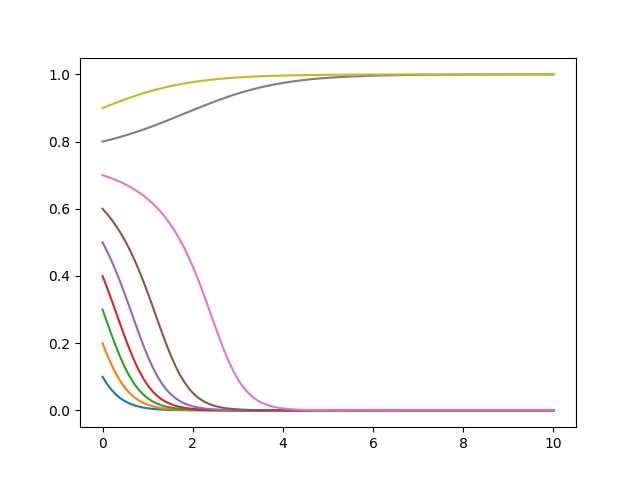
\includegraphics[scale=0.5]{basinofattraction.pdf}
        \caption[Replicator dynamic of the stag hunt game]{Replicator dynamics in the stag hunt game for 
                $\alpha_1=1,\ \alpha_2=3$ with different initial conditions}
                \label{fig:basinofattraction}
\end{figure}

Concerning the equilibrium selection, the evolutionary approach with replicator
dynamic has a definite answer. The population will reach one of the three
Nash equilibria depending on the initial condition. 
However, an equilibrium that is not asymptotically stable 
is rather implausible,
because it only emerges from one initial condition in which the population
is already exactly in that population state. 
Intuitively, one additional agent playing
a pure strategy suffices to get the population state moving to one of the
pure equilibria. As the model outlined here is only a deterministic
approximation, any stochastic shock would lead to such a disturbance and hence
would start convergence to one of the states with evolutionary stable 
strategies.
The population converges to the stag hunting or the hare
hunting equilibrium if the initial conditions lie in their 
basin of attraction.
As discussed earlier, the population converges to the state $x=1$, 
the stag hunting equilibrium of the stage game, for all initial conditions 
$x_0 \in (\frac{\alpha_2}{\alpha_1+\alpha_2},1]$. Any trajectory of the 
dynamical system with initial conditions 
$x_0 \in [0,\frac{\alpha_2}{\alpha_1+\alpha_2})$ leads to the hare hunting
equilibrium. 

Interestingly, one observes another connection of the 
dynamic with the stage game. 
By definition \eqref{eq:riskdom}, 
the hare hunting equilibrium risk-dominates if $\alpha_2 > \alpha_1$.
Thus the basin of attraction is larger for an equilibrium that 
risk-dominates the other. With the parameter setting shown
in figure \ref{fig:basinofattraction}, $75\%$ of the possible initial 
conditions lead to the risk-dominant equilibrium, whereas only $25\%$ of 
them lead to the payoff-dominant equilibrium. This 
connection was for example also shown by \textcite{kandori_learning_1993} 
in a stochastical model. The convergence to the risk-dominant equilibrium
in one dimension was independent of the specific adjustment process 
underlying the dynamic, aslong it satisfied payoff monotonicity. 
However, it is not clear what specifies the 
initial conditions which ultimately determine the selected equilibrium in 
the deterministic case. 
If it is assumed, for example, that agents choose a random strategy 
in a first round of the game independently from each other, 
one can say that the equilibrium with a 
larger basin of attraction, the risk-dominant equilibrium, is reached more 
likely. Otherwise, a ``slice of history'', knowledge about how the population
has played before, is needed to know in which population
state the dynamic starts \parencite{friedman_economic_1998}. 
